% no answer key
\documentclass[letterpaper]{exam}

% answer key
% \documentclass[letterpaper, landscape]{exam}
% \usepackage{2in1, lscape} 
% \printanswers

\usepackage{units} 
\usepackage{xfrac} 
\usepackage[fleqn]{amsmath}
\usepackage{cancel}
\usepackage{float}
\usepackage{mdwlist}
\usepackage{booktabs}
\usepackage{cancel}
\usepackage{polynom}
\usepackage{caption}
\usepackage{fullpage}
\usepackage{comment}
\usepackage{enumerate}
\usepackage{graphicx}
\usepackage{parskip}

\everymath{\displaystyle}


\title{Statistics \\ Homework Eight}
\date{\today}
\author{}

\begin{document}

  \maketitle

  \section{Homework}
    \begin{itemize*}
      \item read Chapter 9 
      \item take a look at the ``Check Your Skills'' exercises
      \item exercises: 29-32, 34, 36, 38-41, 43-44, 48
      \item if you're interested, read the {\em Data Ethics} essay
    \end{itemize*}

  \ifprintanswers
    \begin{description}

      \item[29] 
        This is an experiment.  The explanatory variable is the amount of
        information the interviewer provided and the response variable is
        whether the subject completed the interview.

      \item[30]
        \begin{enumerate}[(a)]
          \item Do students with higher family income tend to get better grades?

          \item Does taking Vitamin B daily improve grades?
        \end{enumerate}

      \item[31]
        \begin{enumerate}[(a)]
          \item In an observational study, the subjects decide whether or not
            they are going to take vitamin E and the researcher observers
            differences in outcomes.  In an experiment, the researcher decides
            which of the subjects will take vitamin E.

          \item A ``randomized controlled trial'' is an experiment in which 
            \begin{itemize*}
              \item some subjects have the treatment and others don't
              \item which subject is which is determined by random chance, with
                each subject having an equal chance to end up in either group
            \end{itemize*}

          \item Yes.People who take vitamin E already probably have other
            healthy habits as well, so they naturally have better health,
            independent of any effect vitamin E might have.
        \end{enumerate}

      \item[32] If we assume that we'll be able to reach all 544 adults, we can
        divide them into two groups in advance.  One group will be read the
        first description and one group will be read the second description.

        Alternate between the groups, calling someone from group A, someone from
        group B, etc. This way you will be obtaining the samples at around the
        same time which will help control for a lurking variable like a current
        event regarding poor people.
        
      \item[34]
        \begin{enumerate}[(a)]
          \item The treatment group is the people with the strong pot and the
            control group is the others.  The subjects are randomly assigned to
            one group or the other.

          \item TO DO
        \end{enumerate}

      \item[36]
        \begin{enumerate}[(a)]
          \item The factors are:
            \begin{itemize*}
              \item roller type (metal or natural-bristle
              \item dyeing cycle time (30 minutes or 40 minutes)
              \item temperature (150 or 175 degrees C)
            \end{itemize*}

           There are 8 combinations of the three variables so 24 subjects
           will be required to get three samples for each combination.

          \item 
            \begin{itemize*}
              \item select 24 pieces of fabric for the test
              \item number the treatments from 1 to 8
              \item shuffle the pieces of fabric around so they are in random
                order
              \item give the first piece treatment 1, the second piece treatment
                2, etc.
              \item measure the results
            \end{itemize*}
        \end{enumerate}

      \item[38]
        \begin{enumerate}[(a)]
          \item There are two kinds of sprays and two kinds of pills, making 4
            different treatments.  

          \item I would assign a unique random number between 1 and 240 to each
            subject.

          \item With numbers random assigned to patients, numbers 1-53 would get
            the steroid spray and the antibiotic pill, numbers 65-117 would get
            the steroid spray and placebo pill, etc.
        \end{enumerate}

      \item[39]
        The factors are the type of spray and the type of pill.

        Double-blind means that neither the subjects nor the person
        administering the pills/sprays nor the subject knows what treatment a
        particular subject is receiving.

        Placebo-controlled means that some of the subjects are given placebos.
        This allows the researcher to compare the effect of the treatment with
        the effect of no treatment without letting the subjects know they
        aren't receiving any actual medicine.

      \item[40] This doesn't mean there was no difference at all.  It just means
        that the differences between the groups was about what you'd expect with
        natural random variation.  None of the groups stood out by having an
        unexpectedly large or small numbers of smokers, for example.

      \item[41] 
        \begin{enumerate}[(a)]
          \item The pairs could be the same person on different days.  You
            wouldn't want to feed someone two beverages in close succession,
            because the reaction to the second one would probably generally be
            different.  
            
            The randomization would be to decide which beverage each subject
            gets first.

          \item Since there are only two treatments, you just have to go through
            the table and if the number is even, assign treatment 1 and if it is
            odd assign treatment 2.  Once you have enough of either treatment,
            assign the remaining samples to the remaining treatment.

            Using table B, the results would be:

            \begin{tabular}[H]{ll}
              \toprule
              treatment     & subjects \\
              \midrule
              Regular first & 2, 4, 9, 10, 11, 13, 14, 15, 17, 18 \\
              Light first   & 1, 3, 5, 6,   7,  8, 12, 16, 19, 20 \\
              \bottomrule
            \end{tabular}
        \end{enumerate}

      \item[43]
        The best thing would be to do the test over two days with the matched
        pair being the same player.  For each player, you would randomly
        determine whether he got oxygen on day one or day two and compare the
        performance on the two days.

        You wouldn't want to do the test twice on the same day, because the
        players would be tired for the second run on each day.

        One problem is the psychological effect receiving oxygen might have on
        the players.  If they think the oxygen is helping, they might run
        faster, even if it isn't actually helping.  On the other hand, the same
        would be true in a game, so as long as the oxygen has an effect,
        psychological or otherwise, it's probably worth using.

      \item[44]
        \begin{figure}[H]
          \centering
          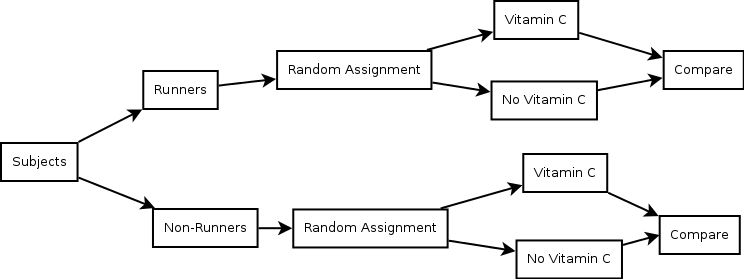
\includegraphics[scale = 0.3]{ex43.png}
          \caption{Exercise 43 (b)}
          \label{fig:ex43}
        \end{figure}
        \begin{enumerate}[(a)]
          \item This is a {\em block design} experiment.

          \item see Figure \ref{fig:ex43}
        \end{enumerate}

      \item[48] 
        \begin{enumerate}[(a)]
          \item The explanatory variables are the vitamins.  The response
            variable is the incidence of colon cancer.

          \item If we had 400 subjects, we could randomly assign each subject to
            one of the 4 treatments.  This would give us 100 subjects per
            treatment.

          \item Neither the subjects nor the people providing the vitamins and
            testing for cancer knew which subject was getting which treatment.

          \item The only differences were the minor differences you would expect
            from random variations in cancer rates.

          \item Here are a few theories:
            \begin{itemize}
              \item There may be something else, like high fiber, in the fruits
                and vegetables which reduces cancer.  

              \item People who eat a lot of fruit and vegetables may not eat
                much of something else (meat, cake, etc.).  They have less
                cancer because they eat less of this cancer-causing food item,
                not because they eat more fruits and vegetables.

              \item People who eat a lot of fruit and vegetables may have other
                unrelated healthy habits like exercising.

            \end{itemize}
        \end{enumerate}
  \end{description}

  \else
    \vspace{10 cm}
    \begin{quote}
      \begin{em}
        % Is a democracy, such as we know it, the last improvement possible in
        % government? Is it not possible to take a step further towards
        % recognizing and organizing the rights of man? There will never be a
        % really free and enlightened State until the State comes to recognize the
        % individual as a higher and independent power, from which all its own
        % power and authority are derived, and treats him accordingly. 
        
        I please myself with imagining a State at least which can afford to be
        just to all men, and to treat the individual with respect as a neighbor;
        which even would not think it inconsistent with its own repose if a few
        were to live aloof from it, not meddling with it, nor embraced by it,
        who fulfilled all the duties of neighbors and fellow-men.
      \end{em}
    \end{quote}
    \hspace{1 cm} --Henry David Thoreau
  \fi

\end{document}

